\chapter{Lecture 7: Topics in String Theory}

These notes follow Leonard Susskind's seventh lecture in the supplementary Winter 2011 string-theory track of \emph{Cosmology and Black Holes}, curated by LazyingArt LLC. The lecture does not begin anew; it returns to an unfinished question from the previous meeting, assembles a small collection of simple equations, and then uses them to give a parametric explanation of black-hole entropy. From there the discussion broadens into the holographic principle and ends with a deliberate turn toward cosmology, where the metric of an expanding universe and the exponentially expanding de Sitter solution are introduced as the bridge to the next lecture.

\section{Recap and the Target Problem}

Susskind begins by going back to the string-counting discussion from the previous lecture. A brief question from the room settles one remaining point: identical small strings are treated as indistinguishable when they have the same length, but their positions in the box are still counted. The box, however, is taken to be of the size occupied by the corresponding single long string. The lecture therefore reopens not with a reset, but with one last clarification of the counting problem that motivated the whole story.

Only after that does he state the real plan. He wants first to write a few equations on the board, all of them simple, and only then to set the target: a derivation of the entropy of a black hole from string theory. He emphasizes the tone of the exercise. The argument is mathematically easy, almost embarrassingly easy, but conceptually subtle. It is precisely the sort of derivation that uses very little formal machinery and yet depends on getting the sequence of ideas exactly right.

\section{Natural Units and the Planck--String Relation}

The first step is dimensional bookkeeping. Susskind adopts natural units,
\begin{equation}
c=\hbar=1,
\end{equation}
while keeping Newton's constant explicit. In these units length and time are measured in the same units, and the immediate question is: what dimensions do mass and \(G_N\) carry?

\begin{figure}
\centering

\includegraphics[width=0.56\textwidth]{lecture_07_figure_02.png}
\caption{Natural-units setup for the energy relation. The board visibly shows only \(c=\hbar=1\) and the starting symbol \(E\); the nearby formulas are the cleaned reconstruction of the dimensional argument that the lecture proceeds to make.}
\end{figure}

The board image captures only the beginning of the argument, so the transcript has to complete it. The intended chain is
\begin{align}
E &\sim \frac{\hbar c}{\lambda}, \\
m &= \frac{E}{c^2}.
\end{align}
Once \(c=\hbar=1\), this becomes
\begin{equation}
m \sim \frac{1}{\lambda}.
\end{equation}
Thus mass has the dimensions of inverse length.

The discussion is verbally loose at this point, but the mathematical point is clear: in natural units one may trade a mass scale for an inverse length scale. This is the unit conversion that will later make both the string formulas and the black-hole formulas intelligible.

The dimensions of Newton's constant are extracted from the simplest gravitational relation on the board,
\begin{equation}
a \sim \frac{G_N M}{R^2}.
\end{equation}
In the chosen units,
\[
[a]\sim \frac{L}{T^2}\sim \frac{1}{L}, \qquad [M]\sim \frac{1}{L}, \qquad [R^2]\sim L^2,
\]
and therefore
\begin{equation}
[G_N]=L^2.
\end{equation}
So Newton's constant has the dimensions of an area. The transcript loosely says that \(G\) is ``the Planck area squared,'' but the mathematically consistent statement is
\begin{equation}
G_N=\ell_p^2.
\end{equation}
That is the form that will be used in the notes.

This already explains why the entropy of a black hole is naturally an area measured in Planck units. But Susskind immediately adds a second fact: \(G_N\) is not only an area, it is also the strength of gravity. He now rephrases gravity in string-theoretic language. The lecture does not attempt a full derivation; it only uses a cartoon. Strings split and rejoin with amplitude \(g_s\), so exchanging a graviton between two bodies brings in two powers of the string coupling. Thus gravitational strength scales as \(g_s^2\).

That cannot be the whole story, because \(g_s\) is dimensionless whereas \(G_N\) carries dimensions of area. The missing factor must come from the fundamental string length \(\ell_s\), the size of the elementary wiggles of a long string. The only sensible scaling relation is therefore
\begin{equation}
G_N \sim g_s^2 \ell_s^2,
\end{equation}
or, taking square roots,
\begin{equation}
\ell_p \sim g_s \ell_s.
\end{equation}
This is the crucial bridge between the gravitational and string-theoretic columns of the lecture: weakening the string coupling makes gravity weak and drives the Planck length far below the string length.

\section{Long Strings as Random Walks}

Only after these scales have been fixed does the lecture turn to string entropy. The motivation is deliberately concrete. Entropy counts decisions needed to specify a configuration. In the crude but useful lattice model Susskind has in mind, a long excited string is replaced by a chain of links. At each vertex the string continues in one of a few allowed directions. In two spatial dimensions, for example, one may picture four possible directions at each step. The exact combinatorial factor is not the point; what matters is that the number of elementary decisions is proportional to the number of steps.

\begin{figure}
\centering

\includegraphics[width=0.42\textwidth]{lecture_07_figure_03.png}

\vspace{1em}

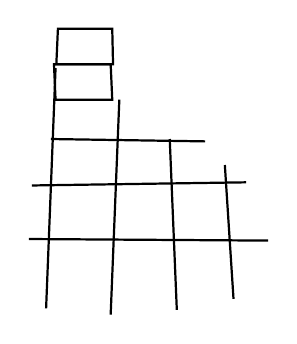
\begin{tikzpicture}[x=1cm,y=1cm]
\draw[line width=0.8pt] (-0.10,-0.10) -- (0.02,2.95);
\draw[line width=0.8pt] (0.72,-0.18) -- (0.83,2.55);
\draw[line width=0.8pt] (1.56,-0.12) -- (1.47,2.05);
\draw[line width=0.8pt] (2.28,0.02) -- (2.17,1.72);

\draw[line width=0.8pt] (-0.32,0.78) -- (2.72,0.76);
\draw[line width=0.8pt] (-0.28,1.46) -- (2.44,1.50);
\draw[line width=0.8pt] (-0.04,2.05) -- (1.92,2.02);

\draw[line width=0.8pt] (0.02,2.55) -- (0.74,2.55) -- (0.72,3.00) -- (0.00,3.00) -- cycle;
\draw[line width=0.8pt] (0.03,3.00) -- (0.75,3.00) -- (0.74,3.45) -- (0.05,3.45) -- cycle;
\end{tikzpicture}
\caption{Rough lattice sketch for the string random walk. The screenshot keeps the original board evidence; the redraw keeps only the discrete, uneven, random-walk character of the picture and does not claim a unique combinatorial construction.}
\end{figure}

The figure is helpful precisely because it is not polished. The string is being modeled as a random walk, and the lecture wants the step size, not the geometric smoothness, to be the central object. If \(\ell_s\) is the size of one elementary step and \(L\) is the total length of the string, then the number of steps is \(L/\ell_s\). Since entropy is the count of such elementary decisions,
\begin{equation}
S_{\mathrm{str}} \sim \frac{L}{\ell_s}.
\end{equation}

This formula is not merely dimensional. It is motivated by the random-walk picture: the entropy is the number of primitive choices needed to specify the walk. The point of introducing the lattice model is to make that statement feel counted rather than declared.

The mass of the string is built in the same way. The total mass is the sum of the masses of the elementary segments. The lecture briefly acknowledges that this is a mild oversimplification, since the kinetic and potential contributions are being compressed into a single effective statement, but Susskind insists that for the scaling argument it is correct in the end.

An elementary segment has length \(\ell_s\). Because mass scales as inverse length in natural units, its mass scale must be
\begin{equation}
m_{\mathrm{seg}} \sim \frac{1}{\ell_s}.
\end{equation}
There are \(L/\ell_s\) such segments, so the total mass of the long string is
\begin{equation}
M \sim \frac{L}{\ell_s}\, m_{\mathrm{seg}} \sim \frac{L}{\ell_s^2}.
\end{equation}
Equivalently,
\begin{equation}
L \sim M \ell_s^2.
\end{equation}
Substituting into the entropy formula gives the compact relation Susskind wants ready for comparison:
\begin{equation}
S_{\mathrm{str}} \sim M\ell_s.
\end{equation}

The lecture has now assembled its string-side formulas. Only now does Susskind say that he wants to compare them with black-hole physics.

\section{First Comparison with Black-Hole Entropy}

At the moment the comparison begins, the board carries a string-theory column whose organization is itself worth preserving.

\begin{figure}
\centering

\includegraphics[width=0.56\textwidth]{lecture_07_figure_04.png}
\caption{String-side equations before the black-hole comparison. The lower mass relation is partly hidden on the board, so the nearby typeset formulas supply the cautious completion justified by the transcript.}
\end{figure}

The visible board organization is well summarized by the cleaned block
\begin{align}
\ell_p &= g_s\ell_s, \\
S_{\mathrm{str}} &= \frac{L}{\ell_s}=M\ell_s, \\
M &= \frac{L}{\ell_s^2}.
\end{align}
As written on the board these appear as equalities; in the surrounding discussion, as throughout the lecture, order-one numerical factors are being suppressed.

The black-hole side begins with the Bekenstein--Hawking formula
\begin{equation}
S_{\mathrm{BH}}=\frac{A}{4G_N}.
\end{equation}
Susskind immediately says that the factor \(1/4\) is not what this argument will compute. What matters first is the scaling:
\begin{equation}
S_{\mathrm{BH}} \sim \frac{A}{G_N} \sim \frac{A}{\ell_p^2}.
\end{equation}
Using the Schwarzschild scaling
\begin{equation}
R_s \sim M G_N,
\end{equation}
one finds
\begin{equation}
A \sim R_s^2 \sim M^2 G_N^2,
\end{equation}
and therefore
\begin{equation}
S_{\mathrm{BH}} \sim M^2 G_N \sim M^2\ell_p^2.
\end{equation}

The comparison is now explicit:
\[
S_{\mathrm{str}} \sim M\ell_s,
\qquad
S_{\mathrm{BH}} \sim M^2\ell_p^2.
\]
The lecture pauses here because this is where the temptation to make a wrong move is strongest. One sees similarity, but also a mismatch. Strings measure entropy in units of length; black holes measure it in units of area. The resemblance is real, but so is the discrepancy.

Susskind insists that the discrepancy is not an embarrassment to be hidden. It is the whole point. If one naively treated the black hole as a free long string, one would simply be ignoring self-gravity. That is the missing ingredient. A gravitating system is not like a gas placed in an externally chosen box; gravitational attraction changes the size of the object and lowers its energy. To make the point vivid, Susskind compares the mistake to modeling a star by taking the same amount of hot matter and putting it in a box larger than the star. One would miss the gravitational attraction that compresses the star and changes its entropy-energy relation. In the same way, the free-string formula misses the self-interaction that squeezes the long string into a black hole.

The lecture therefore changes strategy. Instead of asking whether the original black hole can be treated directly as a string, it introduces a reversible process that moves from one regime to the other.

\section{The Adiabatic Correspondence Between Strings and Black Holes}

This is the conceptual center of the lecture. Susskind's move is to replace a static comparison by what he explicitly calls a game. Take a highly excited string and turn gravity on: it collapses into a black hole. Start with the black hole and turn gravity off: it must eventually become string-like again. In string theory this is meaningful because the coupling \(g_s\) can be varied while the fundamental string length \(\ell_s\) is held fixed.

The small-coupling limit is especially important. If \(g_s\) is taken to zero, the probability for splitting and joining vanishes, which is the same as turning gravity off. In that limit the object can only become a configuration of strings, and the earlier long-string counting problem tells us that the overwhelming majority of such configurations is a single long string rather than many short ones.

The process is to be carried out slowly. That is what makes entropy the relevant invariant. Susskind appeals to the thermodynamic statement that entropy is an adiabatic invariant: under sufficiently slow change of parameters, the entropy remains fixed.

There is one more preparatory step. Before one uses the final black-hole formula, one can still say that the entropy of a large black hole must be a function of the only dimensionless combination available on the gravity side,
\begin{equation}
S_{\mathrm{BH}} = f(M\ell_p).
\end{equation}
At fixed \(\ell_s\), and using \(\ell_p \sim g_s\ell_s\), constant entropy therefore means constant \(Mg_s\). If \((M_0,g_{s,0})\) denotes the original target black hole, the isentropic curve obeys
\begin{equation}
Mg_s = M_0 g_{s,0}.
\end{equation}
This is one of the two curves in the parameter-space picture that Susskind draws on the board. He emphasizes a physical consequence at once: as \(g_s\) is decreased, the negative gravitational binding energy is removed, so the total mass increases. The black hole grows as gravity is weakened.

The second curve marks the crossover from black-hole behavior to string behavior. The lecture does not claim a sharp transition. Instead it adopts the natural criterion that the Schwarzschild radius has shrunk down to the string scale,
\begin{equation}
R_s \sim \ell_s.
\end{equation}
Since \(R_s \sim MG_N\), this gives
\begin{equation}
MG_N \sim \ell_s.
\end{equation}
Using \(G_N \sim g_s^2\ell_s^2\), one arrives at the transition curve
\begin{equation}
Mg_s^2 \sim \frac{1}{\ell_s}.
\end{equation}

At this point the lecture would like the reader to visualize two curves in the \((g_s,M)\) plane: an adiabat \(Mg_s=\text{const}\), and a transition curve \(Mg_s^2\sim 1/\ell_s\). There is no validated frame of the finished graph among the selected images, so the cleanest way to preserve the argument is to carry it algebraically.

\paragraph{The crossover computation.}
Let \((M_\ast,g_{s,\ast})\) be the point where the adiabat meets the transition curve. Then
\begin{align}
M_\ast g_{s,\ast} &= M_0 g_{s,0}, \\
M_\ast g_{s,\ast}^2 &\sim \frac{1}{\ell_s}.
\end{align}
Eliminating \(g_{s,\ast}\) gives
\begin{equation}
g_{s,\ast}=\frac{M_0g_{s,0}}{M_\ast},
\end{equation}
and therefore
\begin{equation}
M_\ast \left(\frac{M_0g_{s,0}}{M_\ast}\right)^2 \sim \frac{1}{\ell_s}.
\end{equation}
Rearranging,
\begin{equation}
M_\ast \ell_s \sim M_0^2 g_{s,0}^2 \ell_s^2.
\end{equation}
Now the factor \(g_{s,0}^2\ell_s^2\) is precisely the original Newton constant \(G_{N,0}\), so
\begin{equation}
M_\ast \ell_s \sim M_0^2 G_{N,0}.
\end{equation}

At the crossover point the object has become string-like, and the string formula applies:
\begin{equation}
S_{\mathrm{str},\ast} \sim M_\ast \ell_s.
\end{equation}
But entropy has not changed along the adiabat, so this is also the entropy of the original black hole:
\begin{equation}
S_{\mathrm{BH}}(M_0) \sim M_0^2 G_{N,0} \sim M_0^2\ell_{p,0}^2.
\end{equation}

This is the intended payoff. The black-hole formula is not obtained by treating the original black hole as a free string. It is obtained by slowly varying the coupling until the black hole becomes string-like, evaluating the entropy where the string description is valid, and then carrying that answer back along a constant-entropy trajectory.

The lecture is equally careful about what this argument does \emph{not} achieve. It does not determine the exact coefficient \(1/4\) in \(A/(4G_N)\). The crossover is not sharp, the location of the transition is only estimated, and the whole discussion works at the level of scaling. What it \emph{does} explain is why black-hole entropy scales as an area in Planck units and why it should be taken seriously as evidence of microscopic substructure.

That historical lesson matters to Susskind. If the answer had come out proportional to \(M^3\ell_p^3\), one would have read it as a volume law, much like ordinary matter in a room or a cup of coffee. Instead the computation reproduces an area law. That is what convinced people that black-hole entropy was not a formal curiosity but a real clue about the microscopic nature of gravity.

\section{Maximum Entropy and the Holographic Principle}

The lecture now pivots from one entropy question to another. The new question is not ``What is the entropy of a black hole?'' but rather ``What is the maximum entropy that can fit in a region of space?''

Susskind first reconstructs the ordinary expectation. Imagine subdividing a room into a lattice of cells. In the simplest toy model, each cell carries one yes-no question: occupied or empty. Then the number of configurations is
\begin{equation}
\Omega = 2^N,
\qquad
N \sim \frac{V}{V_{\mathrm{cell}}},
\end{equation}
and the corresponding entropy is
\begin{equation}
S=\log \Omega \sim \frac{V}{V_{\mathrm{cell}}}\log 2.
\end{equation}
The lecture then corrects itself in the same breath. This is not the entropy of the actual room; it is the \emph{maximum} entropy permitted by that model. The actual room is a low-entropy configuration compared to the completely chaotic state that would saturate the counting bound.

This ordinary reasoning leads one to expect a volume law. The number of independent yes-no decisions scales with the number of cells, hence with the volume. The remarkable claim of the holographic principle is that gravity replaces this by an area law.

Susskind's argument is built from almost nothing. Consider a region of space, taken for simplicity to be spherical, containing total entropy \(S_{\mathrm{initial}}\) and total mass \(M\), with \(M\) smaller than the mass of a black hole whose horizon would just fill the region. If the mass were larger, the black hole would already overflow the boundary.

Now add an incoming shell carrying exactly the extra mass needed to make the whole system collapse into a black hole that fills the region. The shell may be made of anything; only its mass matters. When it falls in, the final state is a black hole of the size of the region. Its entropy is therefore
\begin{equation}
S_{\mathrm{final}}=\frac{A}{4G_N},
\end{equation}
where \(A\) is the area of the boundary of the region.

The second law now does all the work:
\begin{equation}
S_{\mathrm{initial}} \le S_{\mathrm{final}}.
\end{equation}
Hence
\begin{equation}
S_{\mathrm{initial}} \le \frac{A}{4G_N}.
\end{equation}
Since the initial state was arbitrary, this yields the maximal entropy bound
\begin{equation}
S_{\max}=\frac{A}{4G_N},
\end{equation}
or, more cautiously,
\begin{equation}
S_{\max}\le \frac{A}{4G_N}.
\end{equation}

The physical meaning is the same in either form: the number of degrees of freedom that can describe a gravitating region is no larger than the area of its boundary measured in Planck units.

\begin{definition}
The holographic principle is the statement that a region of space may be described by degrees of freedom that scale with the area of its boundary, not with its volume. A convenient way to say this is that there is at most one independent degree of freedom per Planck area on the boundary.
\end{definition}

The lecture dwells on how surprising this is. Locality suggests that independent variations at different interior points should produce a volume law. Gravity instead says that the boundary carries the relevant count. The difference between area and volume in Planck units is enormous for any macroscopic region, so this is not a small correction to familiar intuition; it is a reorganization of it.

\section{Cosmology as the Closing Pivot}

A question from the room now turns the lecture toward cosmology. Susskind explicitly says that he will not write Einstein's equations down; he will simply write a class of solutions. This marks the cosmology segment as a preview rather than a self-contained derivation.

He begins by discussing pictures. The usual balloon analogy for an expanding closed universe is useful, but only up to a point. Taken too literally, it suggests that the ``molecules of space'' get thinned out as the balloon expands. To repair the picture one must imagine that new molecules are inserted so that the local properties of space do not dilute. This prepares the more abstract statement that cosmology is described by a time-dependent metric.

The case chosen for the lecture is spatially flat expanding space,
\begin{equation}
ds^2=-dt^2+a(t)^2\,dx_i dx_i,
\qquad
dx_i dx_i = dx^2+dy^2+dz^2.
\end{equation}
The scale factor \(a(t)\) tells us how proper distances change in time. If two galaxies sit at fixed coordinate separation \(\Delta x\), their proper distance is
\begin{equation}
d(t)=a(t)\,\Delta x.
\end{equation}
Differentiating with respect to time,
\begin{equation}
v=\dot d=\Delta x\,\dot a=\frac{\dot a}{a}\,d.
\end{equation}
This suggests the definition
\begin{equation}
H=\frac{\dot a}{a},
\end{equation}
so that
\begin{equation}
v=Hd.
\end{equation}
This is Hubble's law.

The lecture immediately adds the important caveat that ``Hubble constant'' is a misnomer. In general \(H\) need not be constant in time. What is constant at a given instant is that the same ratio \(v/d\) applies to every pair of comoving points. This is an equal-time statement, not yet a formula for what an observer literally sees when looking backward along the past light cone.

Susskind then points out a consequence that will matter for horizons. In units with \(c=1\), the distance at which recession reaches the speed of light is
\begin{equation}
d_H \sim \frac{1}{H}.
\end{equation}
Objects farther away can recede faster than light without contradicting relativity, because nothing is locally overtaking anything else faster than light; the geometry itself is expanding.

The lecture then isolates the special case in which the Hubble parameter tends to a true constant. In that case,
\begin{equation}
\dot a = Ha,
\end{equation}
and the solution is
\begin{equation}
a(t)=a_0 e^{Ht}.
\end{equation}
The scale factor grows exponentially, and so do proper distances between comoving points. Since the metric contains \(a(t)^2\), the spatial coefficient grows as \(e^{2Ht}\); this is the source of the brief \(2Ht\) remark in the lecture.

A spacetime with this behavior is de Sitter space. The lecture stops at exactly that point. The next step, deferred to the next meeting, is that de Sitter space has a horizon, in a sense complementary to the black-hole horizon: a boundary beyond which objects recede from the observer forever.

\section{Summary}

The lecture unfolds as a sequence of carefully motivated moves. It begins by restoring the previous string-counting problem, then fixes natural units and the relation between Planck and string scales. It next rebuilds the entropy of a long string from the random-walk picture, obtaining \(S_{\mathrm{str}} \sim M\ell_s\), and places that beside the black-hole scaling \(S_{\mathrm{BH}} \sim M^2\ell_p^2\). The mismatch is not swept away; it is used to motivate the real argument, namely the adiabatic interpolation between black holes and strings.

The result is a parametric explanation of why black-hole entropy scales with area in Planck units, together with a clear statement of what that explanation does not compute, namely the exact factor \(1/4\). The lecture then broadens the lesson into the holographic principle, where the maximum entropy of a region is bounded by its boundary area rather than its volume. Finally, after an audience question, it pivots to cosmology and ends with the flat FRW metric, Hubble's law, the scale \(1/H\), and the exponentially expanding de Sitter solution that sets up the next lecture.